\documentclass{beamer}
\mode<presentation> {
%\usetheme{Madrid}
%\usetheme{default}
\usepackage{color}
\definecolor{bottomcolour}{rgb}{0.21,0.11,0.21}
\definecolor{middlecolour}{rgb}{0.21,0.11,0.21}
\setbeamercolor{structure}{fg=white}
\setbeamertemplate{frametitle}[default]%[center]
\setbeamercolor{normal text}{bg=black, fg=white}
\setbeamertemplate{background canvas}[vertical shading]
[bottom=bottomcolour, middle=middlecolour, top=black]
\setbeamertemplate{items}[circle]
\setbeamertemplate{navigation symbols}{} %no nav symbols
\setbeamercolor{block title}{use=structure,fg=white,bg=structure.fg!50!red!50!blue!100!green}
\setbeamercolor{block body}{parent=normal text,use=block title,bg=block title.bg!5!white!10!bg,fg=white}
\setbeamertemplate{navigation symbols}{}
}

\usepackage{graphicx} 
\usepackage{booktabs} 
\usepackage[utf8]{inputenc}  
\usepackage[T1]{fontenc}  
\usepackage{geometry}     
\usepackage[francais]{babel} 
\usepackage{eurosym}
\usepackage{verbatim}
\usepackage{ragged2e}
\justifying

%%%%%%%%%%%%%%%%%%%%%%%%%%%%%%%%%%%%%%%%%%%%%%%%%%%%%%%%%%%%%%%%
%% ccBeamer 0.1, 2007-07-02                                   %%
%% Written by Sebastian Pipping <webmaster@hartwork.org>      %%
%% ---------------------------------------------------------- %%
%% Licensed under Creative Commons Attribution-ShareAlike 3.0 %%
%% http://creativecommons.org/licenses/by-sa/3.0/             %%
%%%%%%%%%%%%%%%%%%%%%%%%%%%%%%%%%%%%%%%%%%%%%%%%%%%%%%%%%%%%%%%%


%% Images
\newcommand{\CcImageBy}[1]{%
	
\includegraphics[scale=#1]{creative_commons/cc_by_30.pdf}%
}
\newcommand{\CcImageCc}[1]{%
	
\includegraphics[scale=#1]{creative_commons/cc_cc_30.pdf}%
}
\newcommand{\CcImageDevNations}[1]{%
	
\includegraphics[scale=#1]{creative_commons/cc_dev_nations_30.pdf}%
}
\newcommand{\CcImageNc}[1]{%
	
\includegraphics[scale=#1]{creative_commons/cc_nc_30.pdf}%
}
\newcommand{\CcImageNd}[1]{%
	
\includegraphics[scale=#1]{creative_commons/cc_nd_30.pdf}%
}
\newcommand{\CcImagePd}[1]{%
	
\includegraphics[scale=#1]{creative_commons/cc_pd_30.pdf}%
}
\newcommand{\CcImageSa}[1]{%
	
\includegraphics[scale=#1]{creative_commons/cc_sa_30.pdf}%
}
\newcommand{\CcImageSampling}[1]{%
	
\includegraphics[scale=#1]{creative_commons/cc_sampling_30.pdf}%
}
\newcommand{\CcImageSamplingPlus}[1]{%
	
\includegraphics[scale=#1]{creative_commons/cc_sampling_plus_30.pdf}%
}


%% Groups
\newcommand{\CcGroupBy}[1]{% zoom
	\CcImageBy{#1}%
}
\newcommand{\CcGroupByNc}[2]{% zoom, gap
	\CcImageBy{#1}\hspace*{#2}\CcImageNc{#1}%
}
\newcommand{\CcGroupByNcNd}[2]{% zoom, gap
	\CcImageBy{#1}\hspace*{#2}\CcImageNc{#1}\hspace*{#2}\CcImageNd{#1}%
}
\newcommand{\CcGroupByNcSa}[2]{% zoom, gap
	\CcImageBy{#1}\hspace*{#2}\CcImageNc{#1}\hspace*{#2}\CcImageSa{#1}%
}
\newcommand{\CcGroupByNd}[2]{% zoom, gap
	\CcImageBy{#1}\hspace*{#2}\CcImageNd{#1}%
}
\newcommand{\CcGroupBySa}[2]{% zoom, gap
	\CcImageBy{#1}\hspace*{#2}\CcImageSa{#1}%
}
\newcommand{\CcGroupDevNations}[1]{% zoom
	\CcImageDevNations{#1}%
}
\newcommand{\CcGroupNcSampling}[2]{% zoom, gap
	\CcImageNc{#1}\hspace*{#2}\CcImageSampling{#1}%
}
\newcommand{\CcGroupPd}[1]{% zoom
	\CcImagePd{#1}%
}
\newcommand{\CcGroupSampling}[1]{% zoom
	\CcImageSampling{#1}%
}
\newcommand{\CcGroupSamplingPlus}[1]{% zoom
	\CcImageSamplingPlus{#1}%
}


%% Text
\newcommand{\CcLongnameBy}{Attribution}
\newcommand{\CcLongnameByNc}{Attribution-NonCommercial}
\newcommand{\CcLongnameByNcNd}{Attribution-NoDerivs}
\newcommand{\CcLongnameByNcSa}{Attribution-NonCommercial-ShareAlike}
\newcommand{\CcLongnameByNd}{Attribution-NoDerivs}
\newcommand{\CcLongnameBySa}{Attribution-ShareAlike}

\newcommand{\CcNote}[1]{% longname
	This work is licensed under the \textit{Creative Commons #1 3.0 License}.%
}


\title[Metadata]{Metadata} 
\author{Genma}

\begin{document}

%% Titlepage
\begin{frame}
	\titlepage
	\vfill
	\begin{center}
		\CcGroupByNcSa{0.83}{0.95ex}\\[2.5ex]
		{\tiny\CcNote{\CcLongnameByNcSa}}
		\vspace*{-2.5ex}
	\end{center}
\end{frame}

%----------------------------------------------------------------------------------------
\begin{frame}
\Huge{\centerline{Metadata}}
\end{frame}

\begin{frame}
\frametitle{Metadata}
\begin{block}{What is metadata?}
\justifying{
Metadata consists of information that characterizes data (e.g. Word documents, pictures, music files, etc). 
\\~\\
In essence, metadata answers who, what, when, where, why, and how about every facet of the data that is being characterized.
}
\end{block}
\end{frame}

%------------------------------------------------

\begin{frame}
\frametitle{Metadata}
\begin{center}
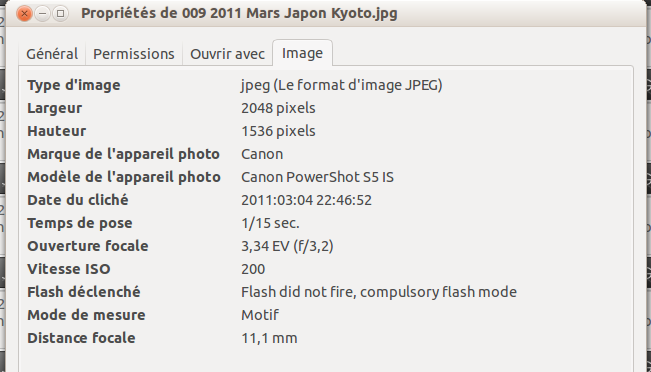
\includegraphics[scale=0.5] {./materials/Metadata.png} 
\end{center}
\end{frame}


%----------------------------------------------------------------------------------------
\begin{frame}
\frametitle{Metadata}
\begin{block}{Why metadata can be a risk for your privacy?}
\justifying{
Metadata within a file can tell a lot about you. 
\\~\\
Cameras record data about when a picture was taken and what camera was used. 
\\~\\
Office documents like pdf or Office automatically add author and company information to documents and spreadsheets. 
\\~\\
Maybe you don't want to disclose this information on the web.
}
\end{block}
\end{frame}

%------------------------------------------------

\begin{frame}
\frametitle{MAT}
\begin{block}{MAT}
\justifying{
Proudly powered by Python, and using Hachoir as much as possible, MAT was originally 
\\~\\
MAT automatically creates a copy of the original documents in a clean version (leaving the original intact
\\~\\
MAT is provided by default in the live-cd Tails.
}
\end{block}
\end{frame}


%------------------------------------------------
\begin{frame}
\frametitle{MAT}

\begin{block}{Currently supported formats}
For now, MAT fully supports the following formats:
\begin{itemize}
\item Portable Network Graphics (.png)
\item JPEG (.jpg, .jpeg, …)
\item Open Documents (.odt, .odx, .ods, …)
\item Office OpenXml (.docx, .pptx, .xlsx, …)
\item Portable Document Fileformat (.pdf)
\item Tape ARchives (.tar, .tar.bz2, …)
\item MPEG AUdio (.mp3, .mp2, .mp1, …)
\item Ogg Vorbis (.ogg, …)
\item Free Lossless Audio Codec (.flac)
\item Torrent (.torrent)
\end{itemize}
\end{block}
\end{frame}

%------------------------------------------------
\begin{frame}
\frametitle{MAT}
\begin{center}
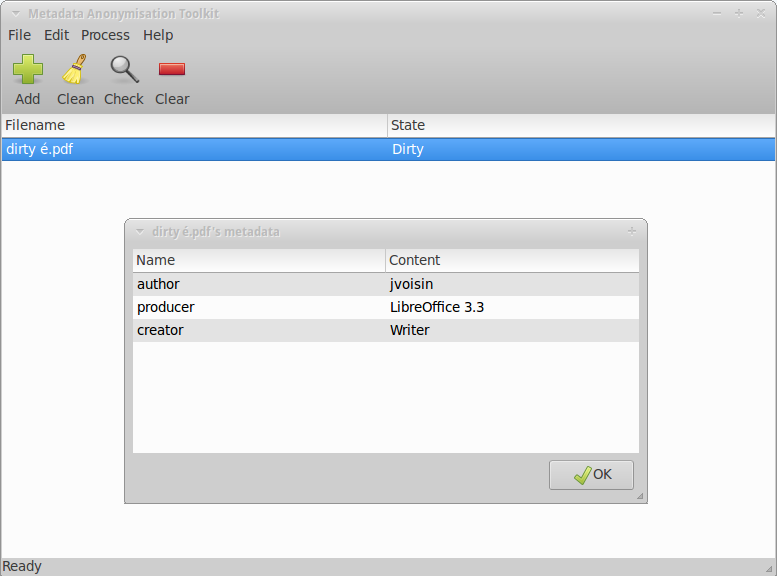
\includegraphics[scale=0.3] {./materials/Mat.png} 
\end{center}
\end{frame}


%----------------------------------------------------------------------------------------
\begin{frame}
\frametitle{MAT}
\begin{block}{Why MAT is not the ultimate solution?}
\justifying{
Mat only removes metadata from your files, it does not anonymise their content, nor handle watermarking, steganography, or any overly customized metadata field/system.

If you really want to be anonymous, use formats that do not contain any metadata, or better: use plain-text. And most important, be careful: every format can be watermarked, even plain text! (e.g. the SNOW project)
}
\end{block}
\end{frame}

%------------------------------------------------
\begin{frame}
\frametitle{Other software}

\begin{block}{Alternatives}
\begin{itemize}
\item Exiftool : \url{http://www.sno.phy.queensu.ca/~phil/exiftool/}
\item exiv2 : \url{http://www.exiv2.org/}
\item jhead : \url{http://www.sentex.net/~mwandel/jhead/}
\item Metanull
\end{itemize}
\end{block}
\end{frame}

\end{document}
